\documentclass[hyperref={unicode}]{beamer}

\usetheme{CambridgeUS}

\usepackage[czech]{babel}
\usepackage[IL2]{fontenc}
\usepackage[utf8]{inputenc}
\usepackage{times}
\usepackage{graphics}

\title{XSS}
\subtitle{Cross-Site Scripting}
\author{Róbert Ďurovič}
\institute{FIT VUT}
\date{\today}

\begin{document}
\begin{frame}
    \titlepage
\end{frame}

\begin{frame}
    \frametitle{Čo je XSS?}
    \begin{itemize}
        \item skratka pre Cross-Site Scripting
        \item druhý najčastejší typ útoku na webe (OWASP)
        \item technika, pri ktorej sa vkladá škodlivý kód do kódu napadnutej webovej aplikácie, ale jej pôvodný kód nie je pozmenený
        \item ovplyvňuje správanie webstránky a zneužíva chyby v prehliadači
        \item využíva sa predovšetkým na kradnutie citlivých údajov
    \end{itemize}    
\end{frame}

\begin{frame}
    \frametitle{Príklad použitia}
    \begin{figure}
        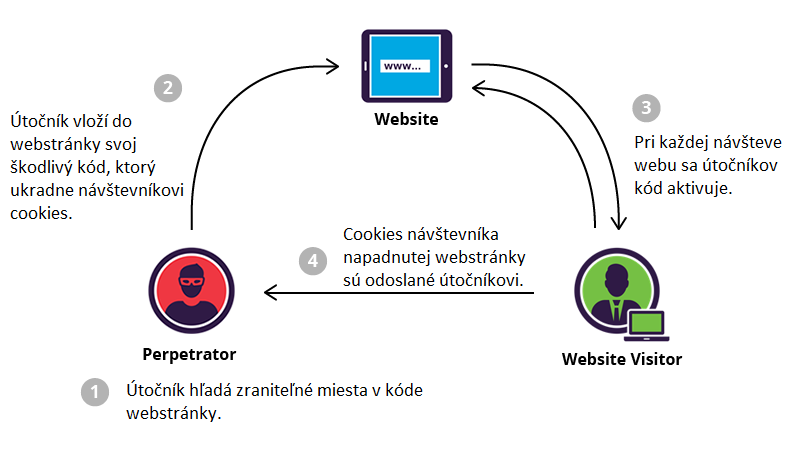
\includegraphics[scale=0.5]{xss.png}
        \caption{Model útoku pomocou XSS}
    \end{figure}
\end{frame}

\begin{frame}
    \frametitle{Typy XSS útokov}
    
    \begin{enumerate}
        \item Perzistentný typ
        \item Neperzistentný typ
        \item Útok s pomocou DOM
    \end{enumerate}
    
    \begin{columns}
    \column{0.5\textwidth}
    \column{0.5\textwidth}
        
\includegraphics[scale=0.5]{injection.jpg}
    \end{columns}
    
\end{frame}

\begin{frame}[fragile]
    \frametitle{Perzistentný typ}
    \begin{itemize}
        \item Uložený priamo vo webovej aplikácii
        \item Typicky v diskusných fórach, chatoch, blogoch atď.
    \end{itemize}
\pause
\textbf{Príklad perzistentného (statického) kódu:}
\begin{semiverbatim}

    <SCRIPT>
        ...
        alert('XSS');
        ...
    </SCRIPT>
\end{semiverbatim}
\end{frame}

\begin{frame}[fragile]
    \frametitle{Neperzistentný typ}
    \begin{itemize}
        \item Kód nie je vo webovej aplikácii pred ani po útoku
        \item Kód je podstrčený obvykle ako parameter URL
        \item Zneužíva zraniteľnosť vyhľadávačov
        \item Šírenie cez správy, emaily alebo cez \texttt{<iframe>}
    \end{itemize}
\pause
\textbf{Príklad použitia neperzistentného (dynamického) kódu:}
\begin{semiverbatim}
  http://search.cz/search.php?dotaz=text<script>
  alert('XSS');</script> 
\end{semiverbatim}
\end{frame}

\begin{frame}[fragile]
    \frametitle{Útok s použitím DOM}
    \begin{itemize}
        \item Document Object Model
        \begin{itemize}
            \item Jazykovo i platformovo nezávislé prostredie
            \item Umožňuje skriptom čítať a meniť obsah, struktúru a štýl dokumentov
        \end{itemize}
        \item Podstatné sú objekty DOM, s ktorými je možné manipulovať, \\napr. \texttt{document.URL} alebo \texttt{document.location}
    \end{itemize}
\pause
\textbf{Príklad útoku s použitím DOM:}
\begin{semiverbatim}
  <SCRIPT>
    var pos=document.URL.indexOf("name=")+5;
    document.write(document.URL
    .substring(pos,document.URL.length));
  </SCRIPT>
\end{semiverbatim}
\end{frame}

\begin{frame}
    \frametitle{Ako sa brániť voči XSS}
    \textbf{Programátori webu:}
        \begin{itemize}
            \item Dôkladne otestovať web na možné bezpečnostné chyby
            \item Využívať bezpečné JavaScript API
        \end{itemize}
    \textbf{Návštevníci webu:}
        \begin{itemize}
            \item Vypnúť JavaScript alebo využívať aplikáciu NoScript
            \item Surfovať iba po zabezpečených weboch
            \item Pri presmerovaní skontrolovať správnosť adresy (phishing)
            \item Byť neustále ostražitý
        \end{itemize}
\end{frame}

\begin{frame}
    \frametitle{Použitá literatúra}
    \begin{itemize}
        \item OWASP: Cross-Site Scripting \\ \texttt{https://www.owasp.org/index.php/XSS}
        \item EXCESS XSS: A comprehensive tutorial on cross-site scripting. \\ \texttt{https://excess-xss.com/}
        \item CHORVÁT, O: Útoky typu Cross-Site Scripting \\
        Bakalářská práce. MUNI, 2010.
        \item OLEJÁR, F.: Analýza útoku vedeného prostředníctvím webového prohlížeče. Bakalářská práce. FIT VUT, 2010.
    \end{itemize}
\end{frame}
\end{document}
